\documentclass[11pt,a4paper]{article}
\usepackage[latin1]{inputenc}
\usepackage{amsmath}
\usepackage{amsfonts}
\usepackage[super,sort&compress,comma]{natbib} 
\usepackage{amssymb}
\usepackage{graphicx}
\usepackage{hyperref}
\author{Andrew R. McCluskey}
\title{ESI for "Probabilistic determination of the effect of a deep eutectic solvent on the structure of lipid monolayers"}
\begin{document}
	
\section{Probability distribution functions}

The two-dimensional probability distribution functions (PDFs) for all parameters and all lipids are given in Figures \ref{fig:dlpc4}-\ref{fig:dmpg5}
\begin{figure}[h]
	\centering
	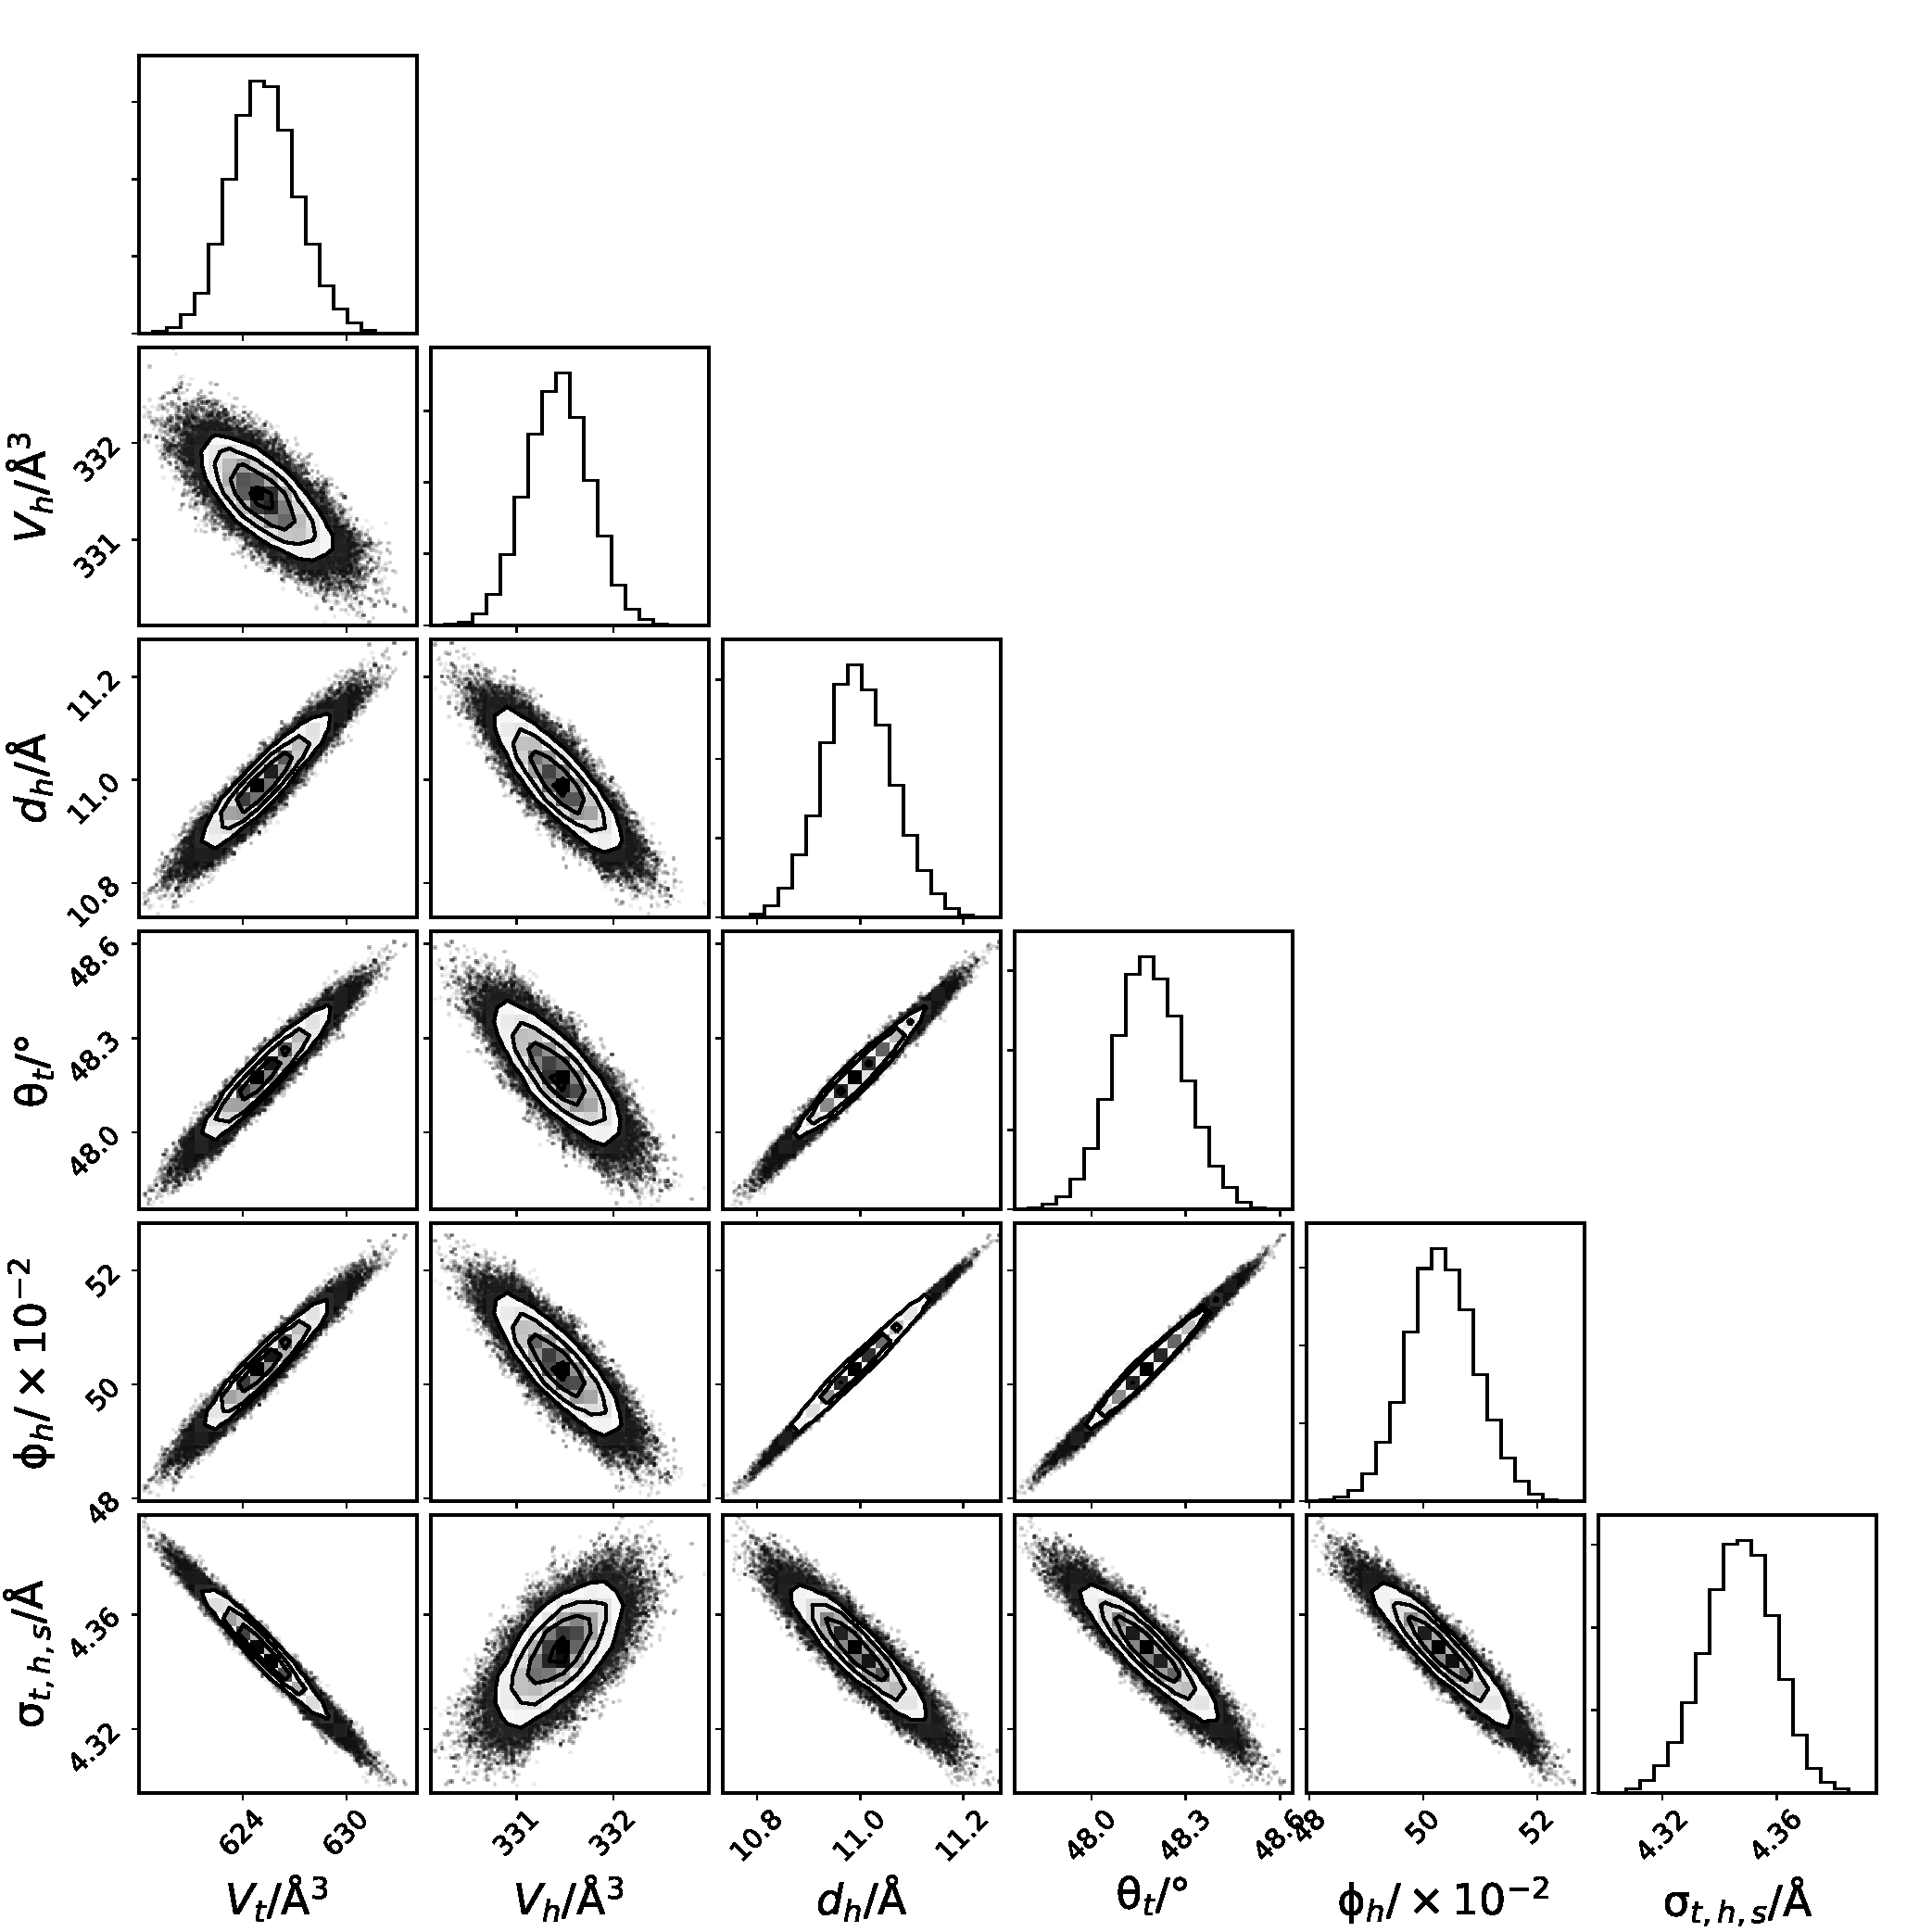
\includegraphics[width=0.50\textwidth]{figures/dlpc4_all_corner}
	\caption{The multi-parameter PDFs for the chemically-relevant model of DLPC reflectometry data at the second-highest concentration. Figure files are available under MIT License.\cite{mccluskey_2018}}
	\label{fig:dlpc4}
\end{figure}
\begin{figure}
	\centering
	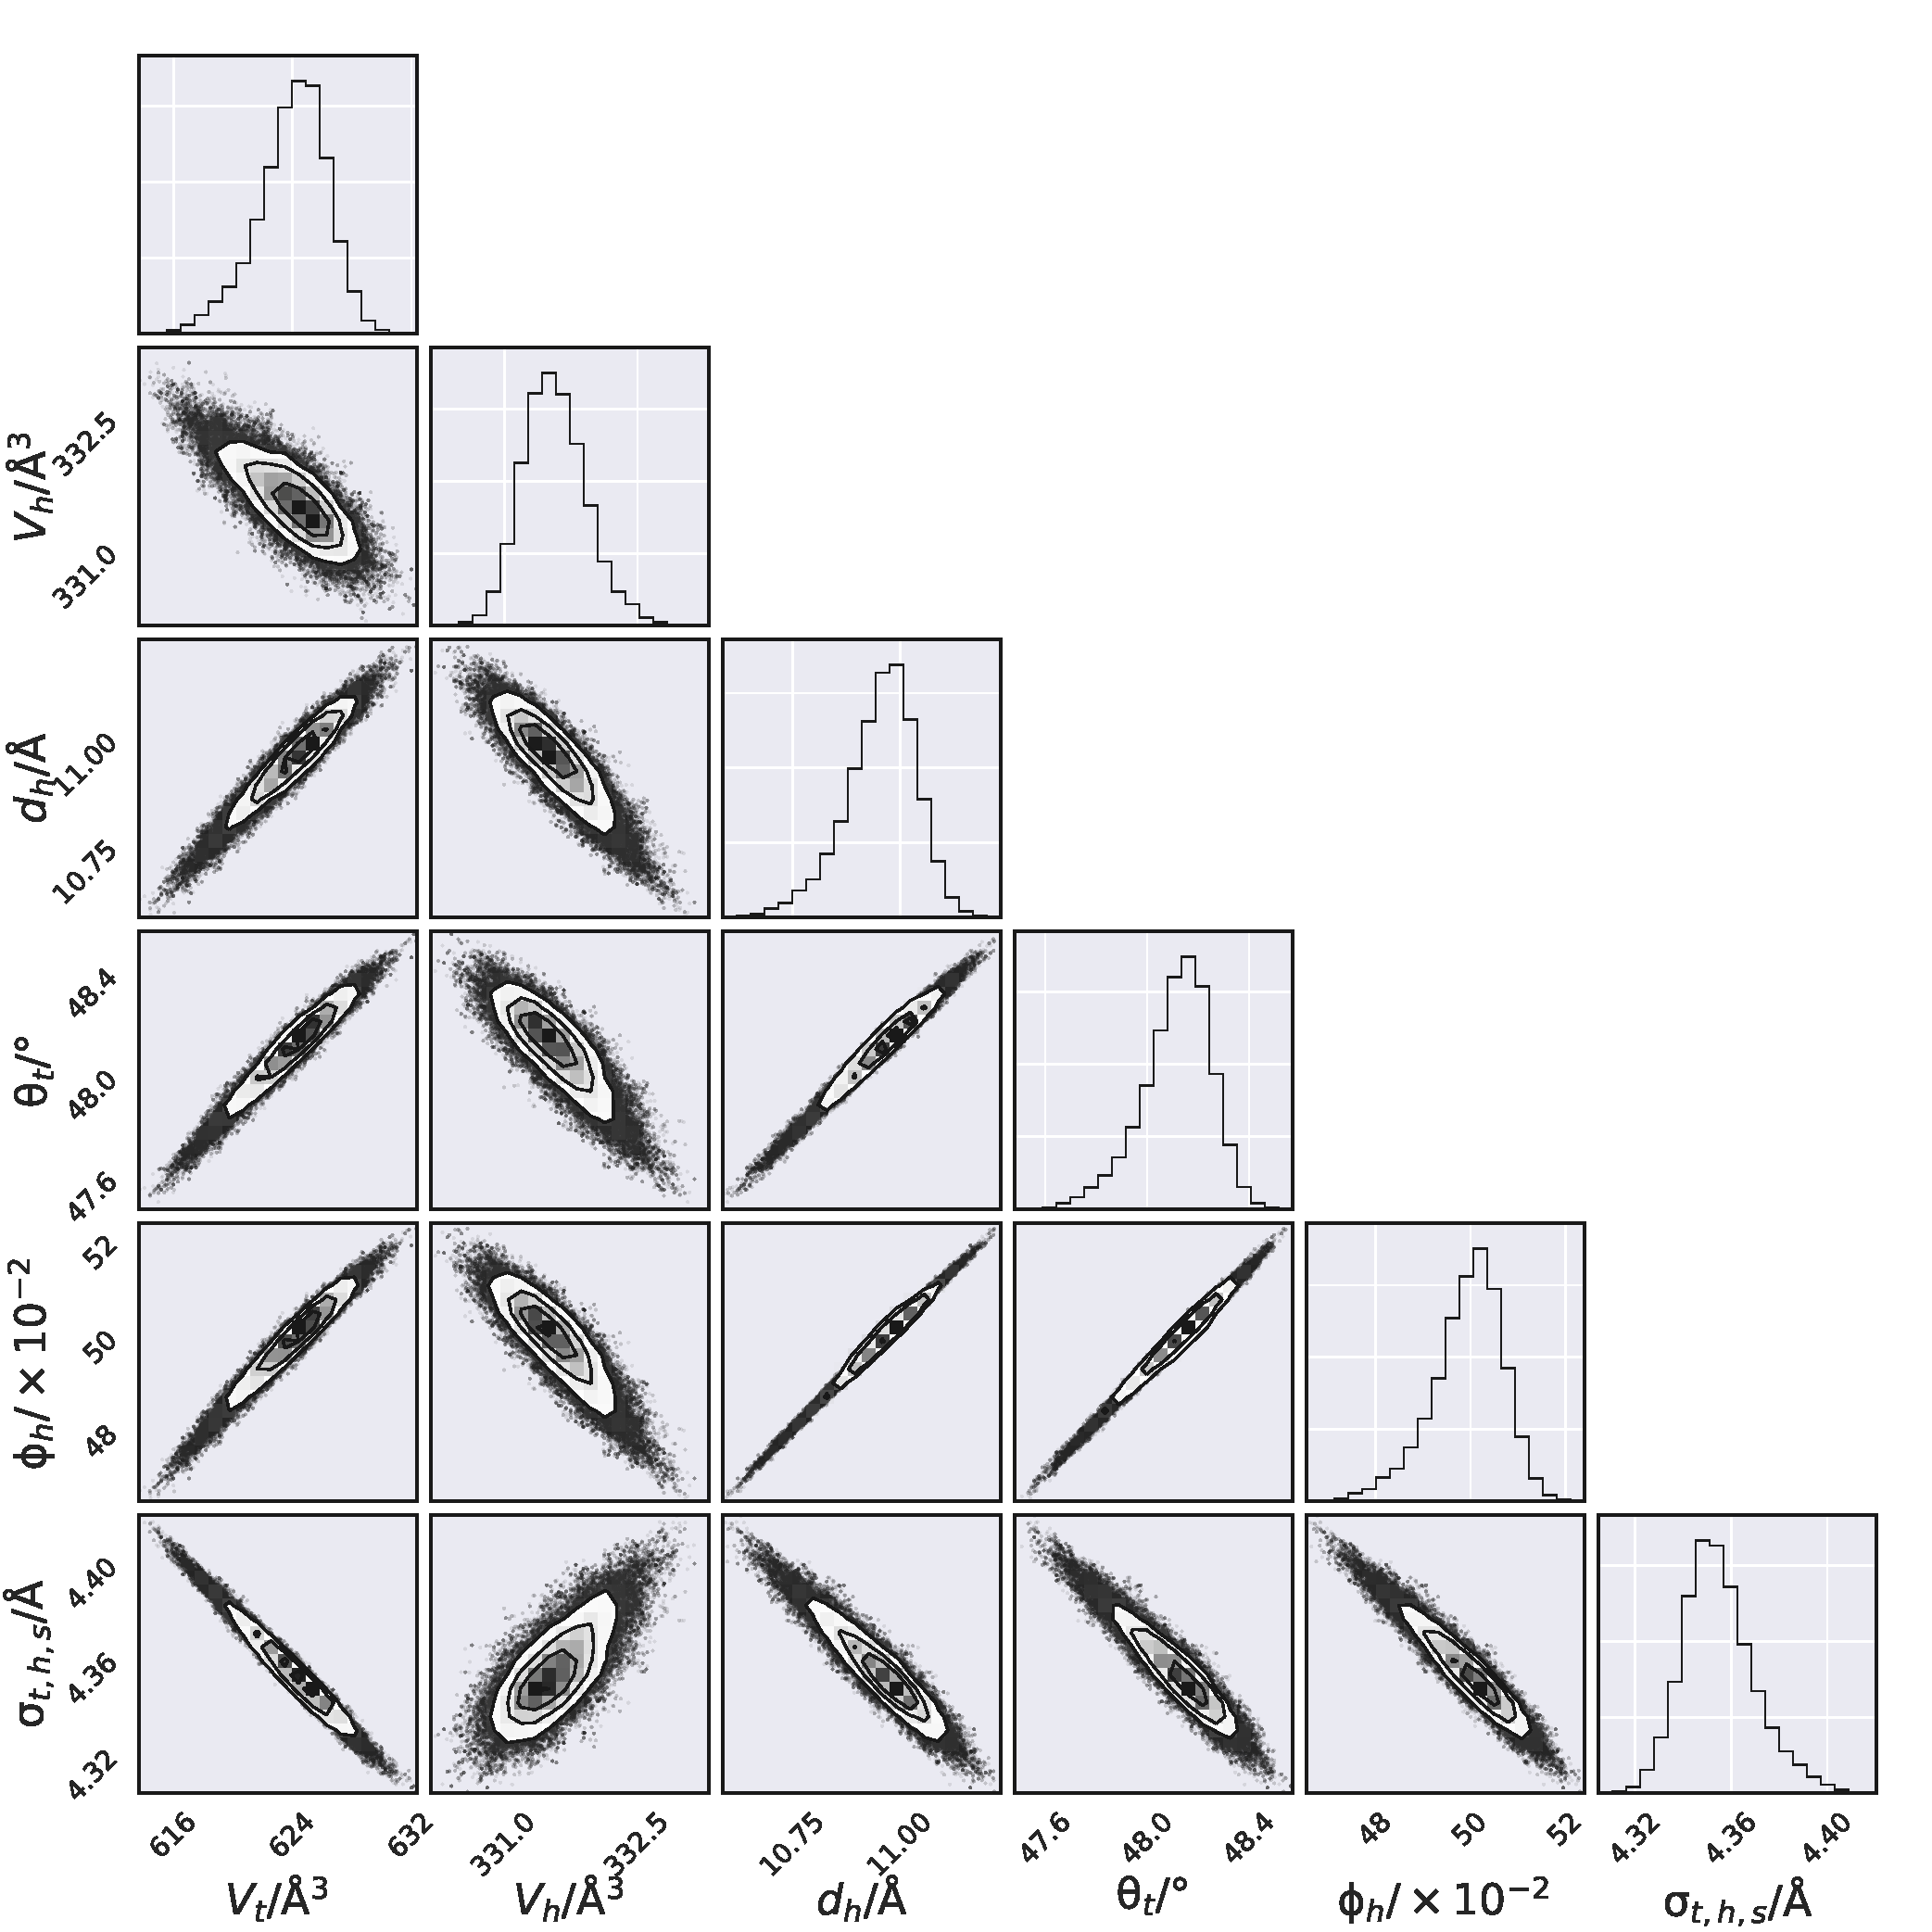
\includegraphics[width=0.50\textwidth]{figures/dlpc5_all_corner}
	\caption{The multi-parameter PDFs for the chemically-relevant model of DLPC reflectometry data at the highest concentration. Figure files are available under MIT License.\cite{mccluskey_2018}}
	\label{fig:dlpc5}
\end{figure}
\begin{figure}
	\centering
	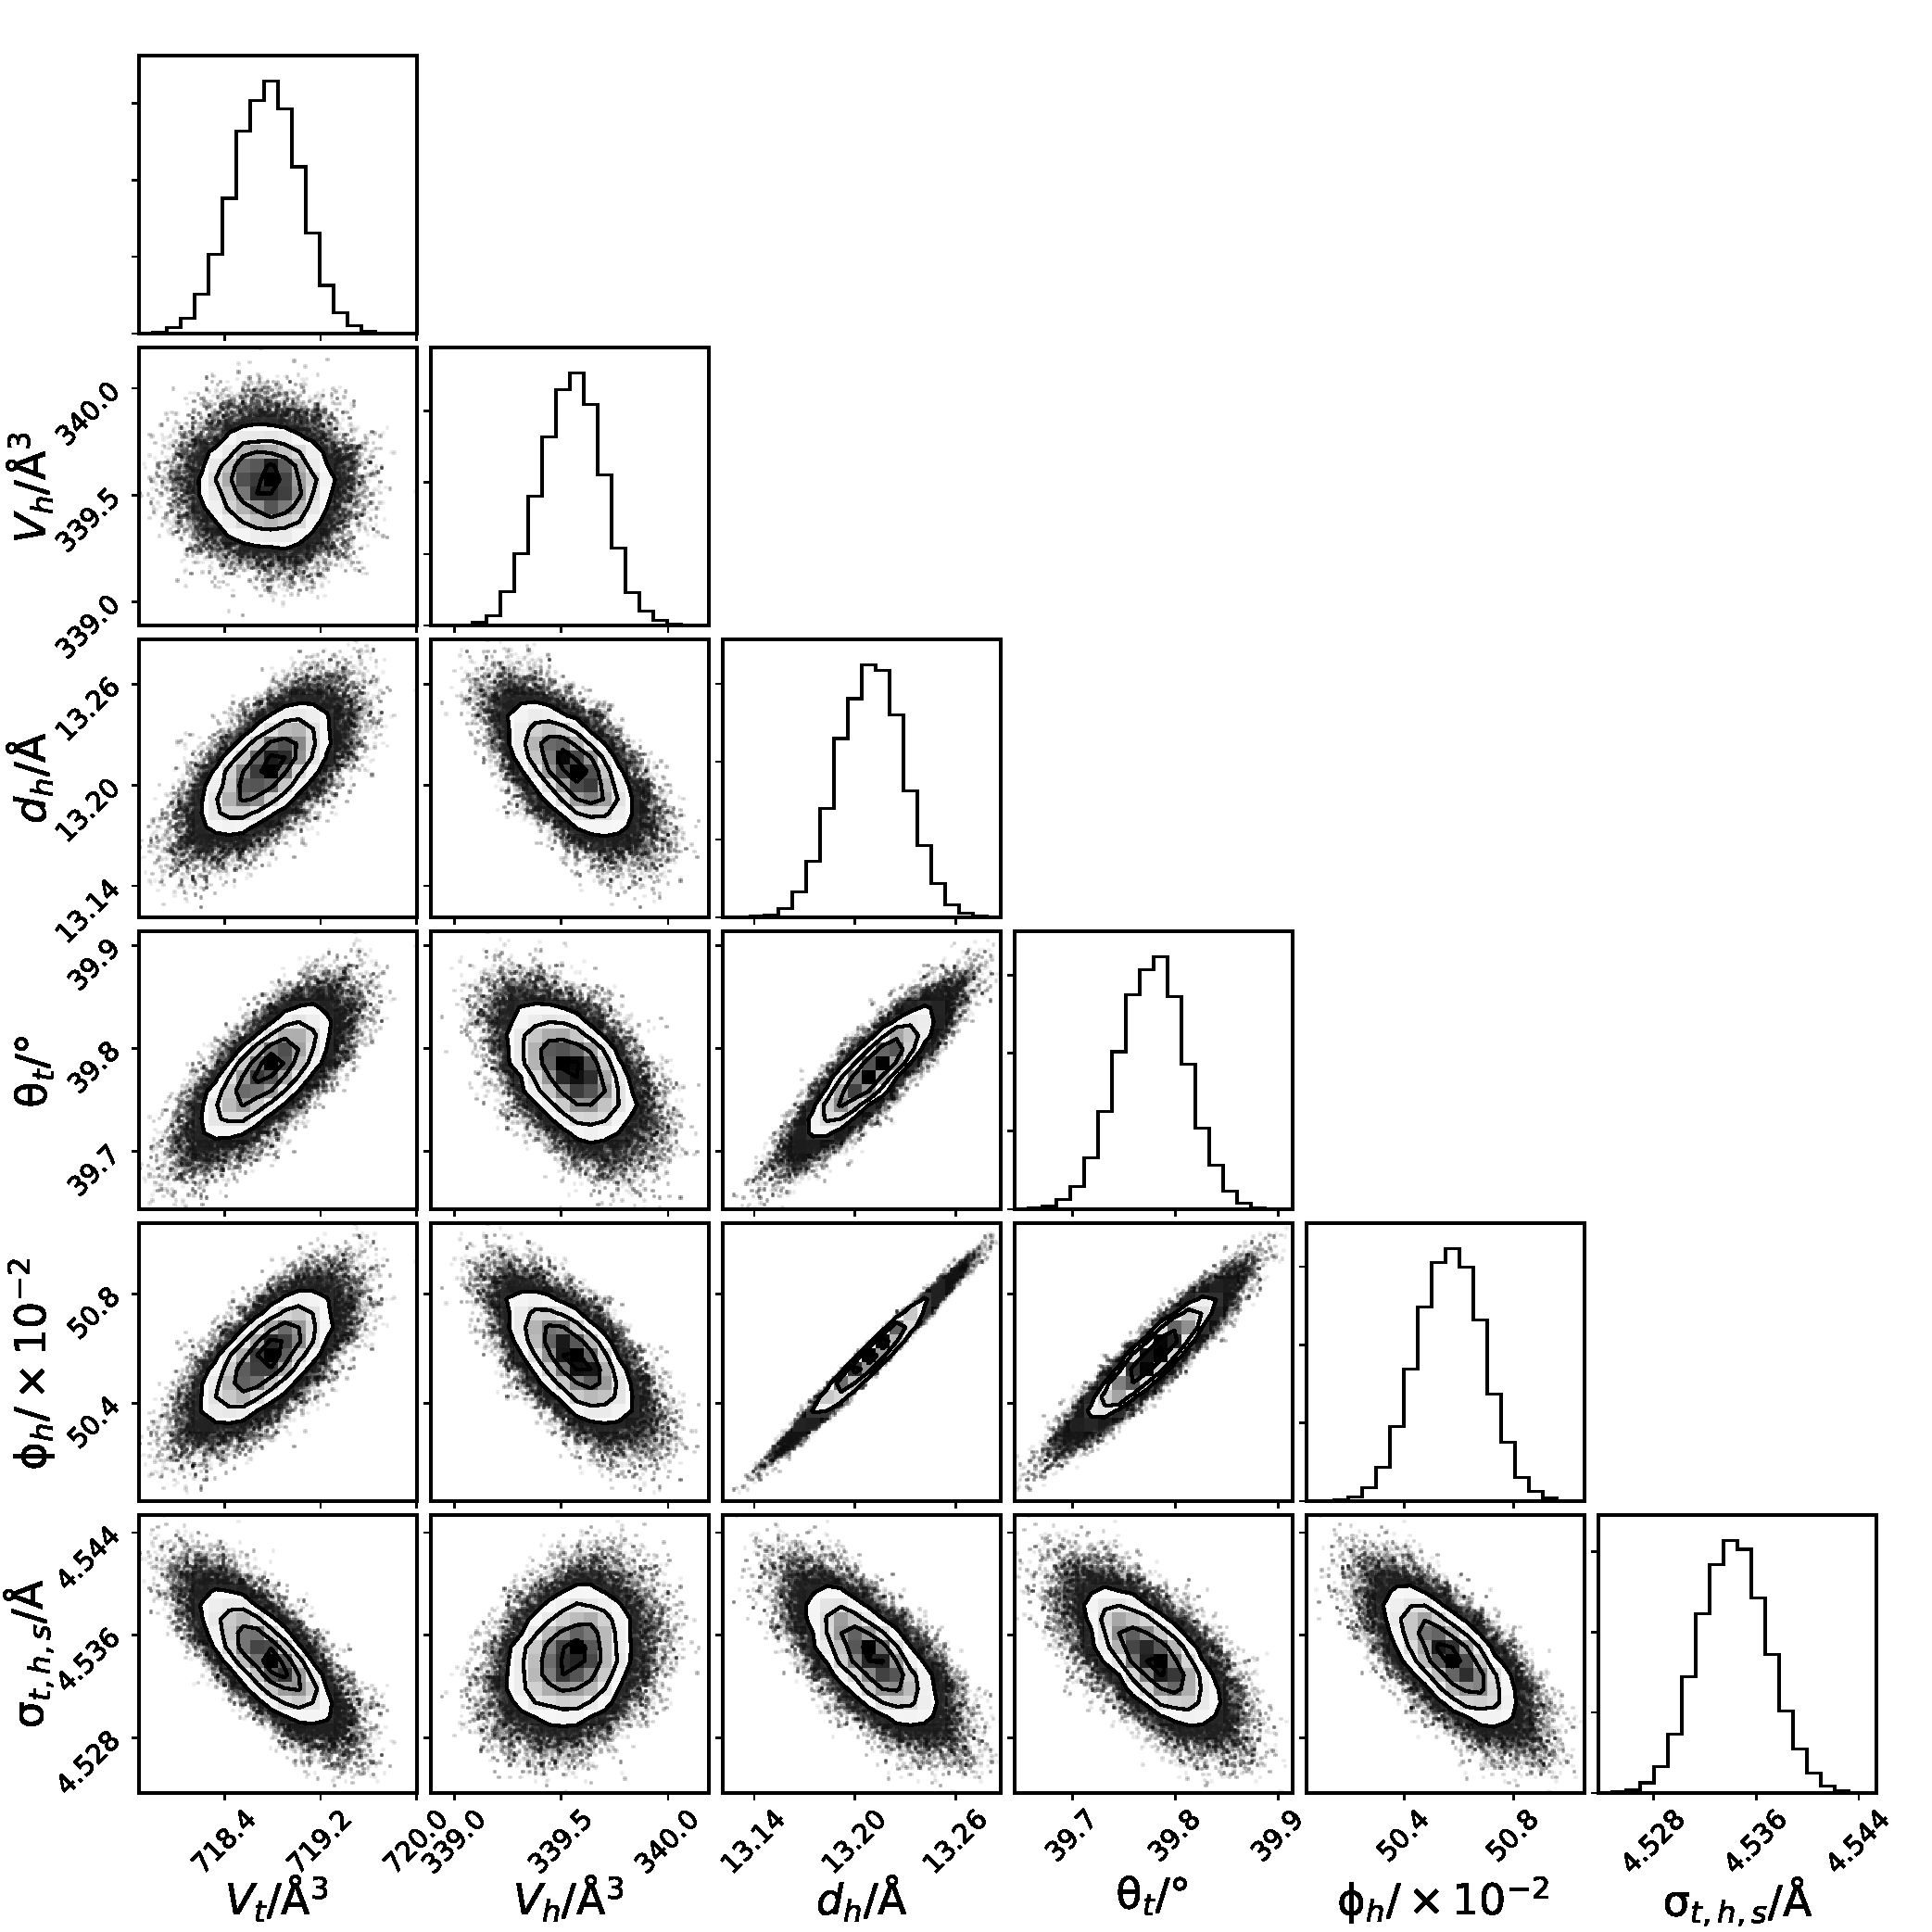
\includegraphics[width=0.50\textwidth]{figures/dmpc4_all_corner}
	\caption{The multi-parameter PDFs for the chemically-relevant model of DMPC reflectometry data at the second-highest concentration. Figure files are available under MIT License.\cite{mccluskey_2018}}
	\label{fig:dmpc4}
\end{figure}
\begin{figure}
	\centering
	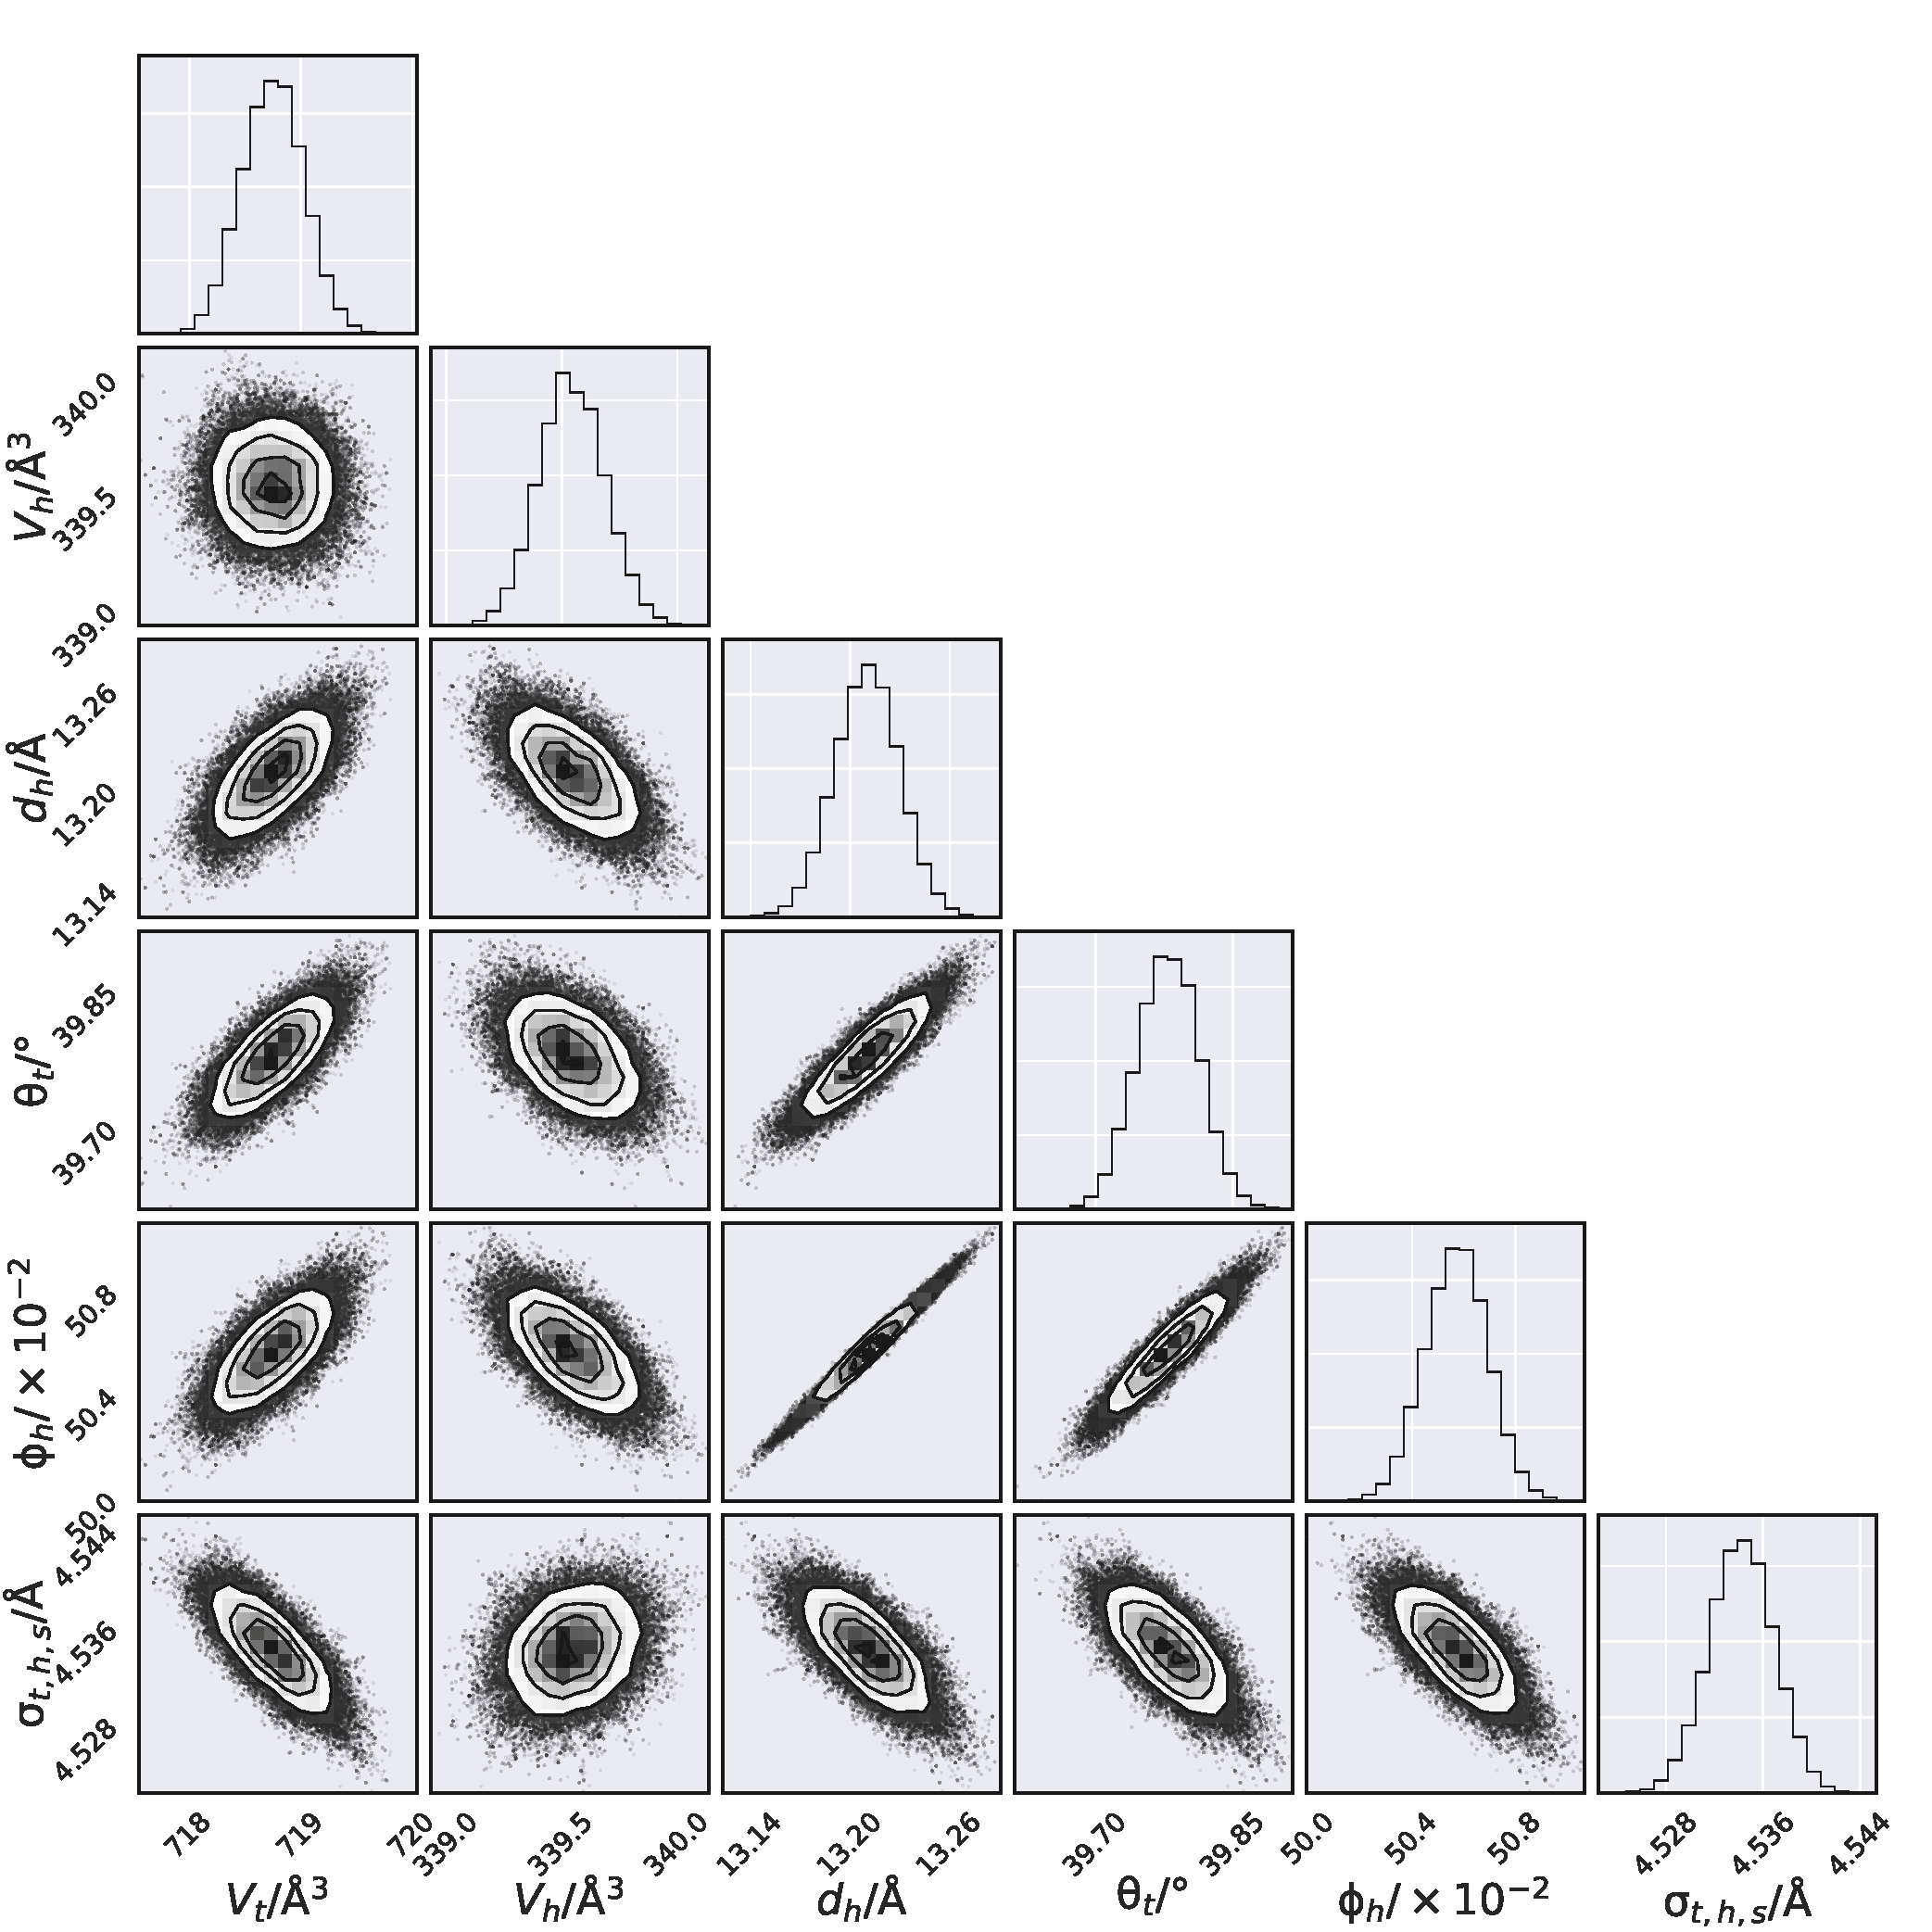
\includegraphics[width=0.50\textwidth]{figures/dmpc5_all_corner}
	\caption{The multi-parameter PDFs for the chemically-relevant model of DMPC reflectometry data at the highest concentration. Figure files are available under MIT License.\cite{mccluskey_2018}}
	\label{fig:dmpc5}
\end{figure}
\begin{figure}
	\centering
	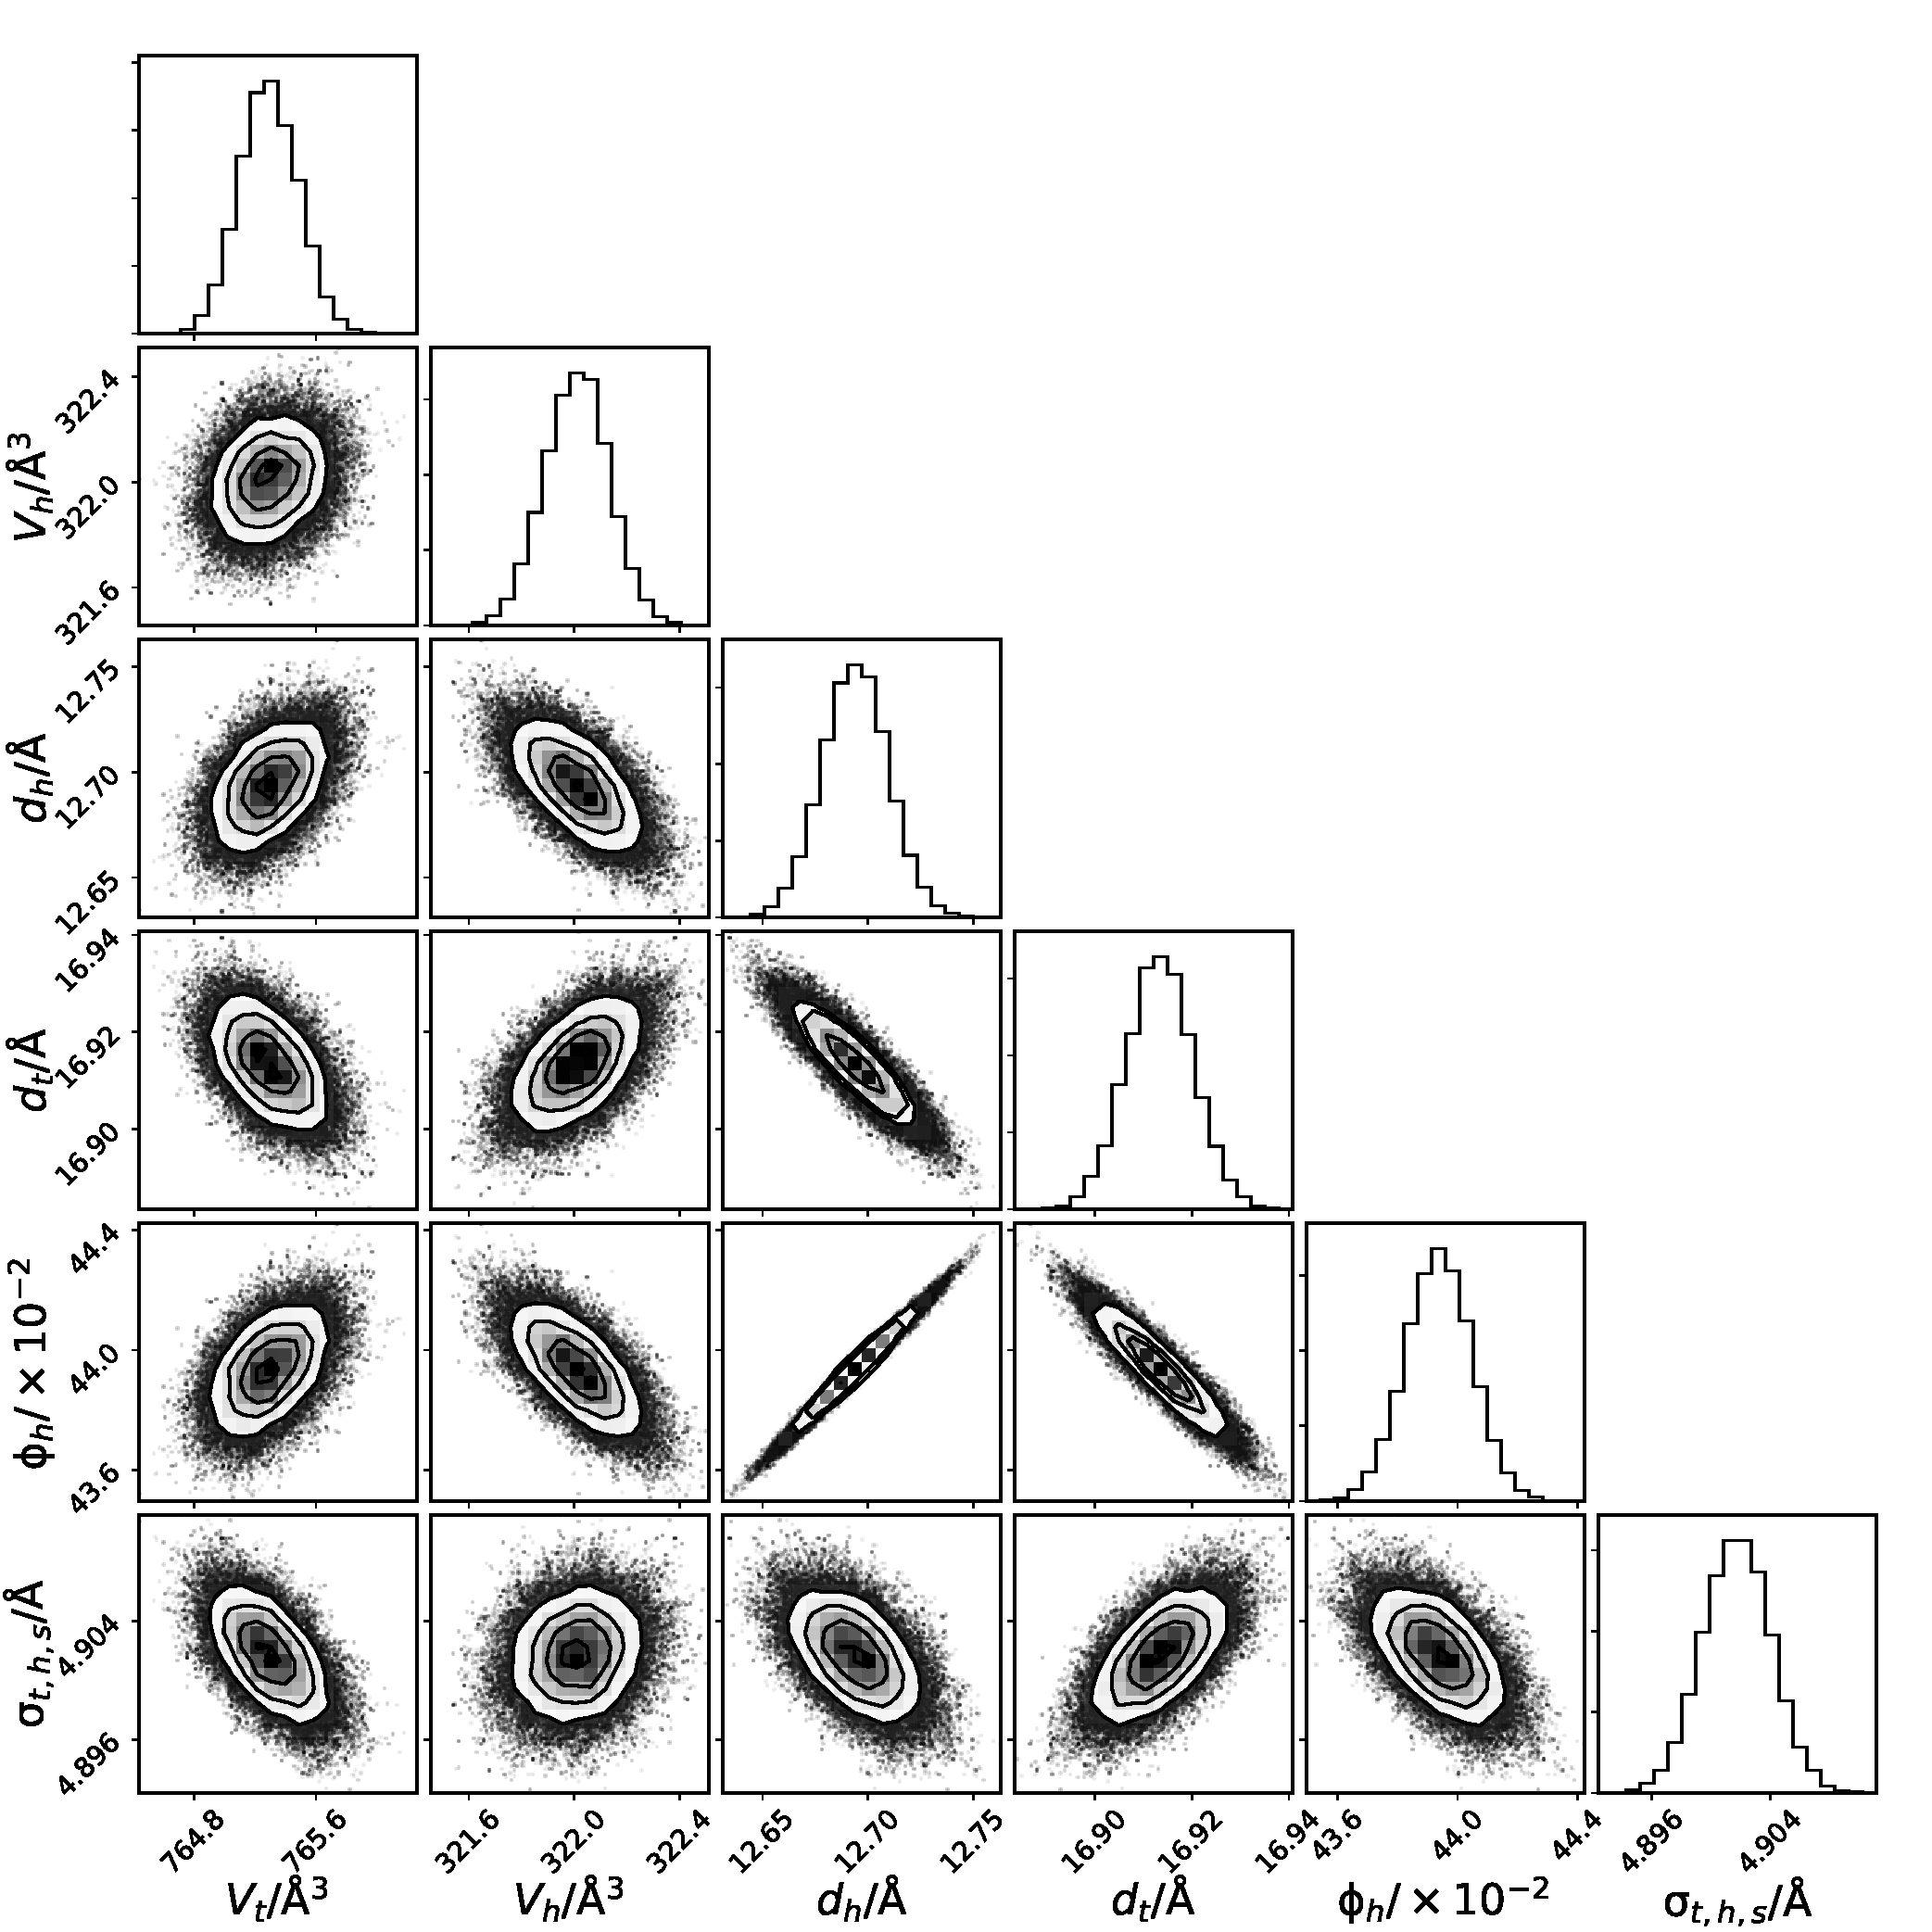
\includegraphics[width=0.50\textwidth]{figures/dppc4_all_corner}
	\caption{The multi-parameter PDFs for the chemically-relevant model of DPPC reflectometry data at the second-highest concentration. Figure files are available under MIT License.\cite{mccluskey_2018}}
	\label{fig:dppc4}
\end{figure}
\begin{figure}
	\centering
	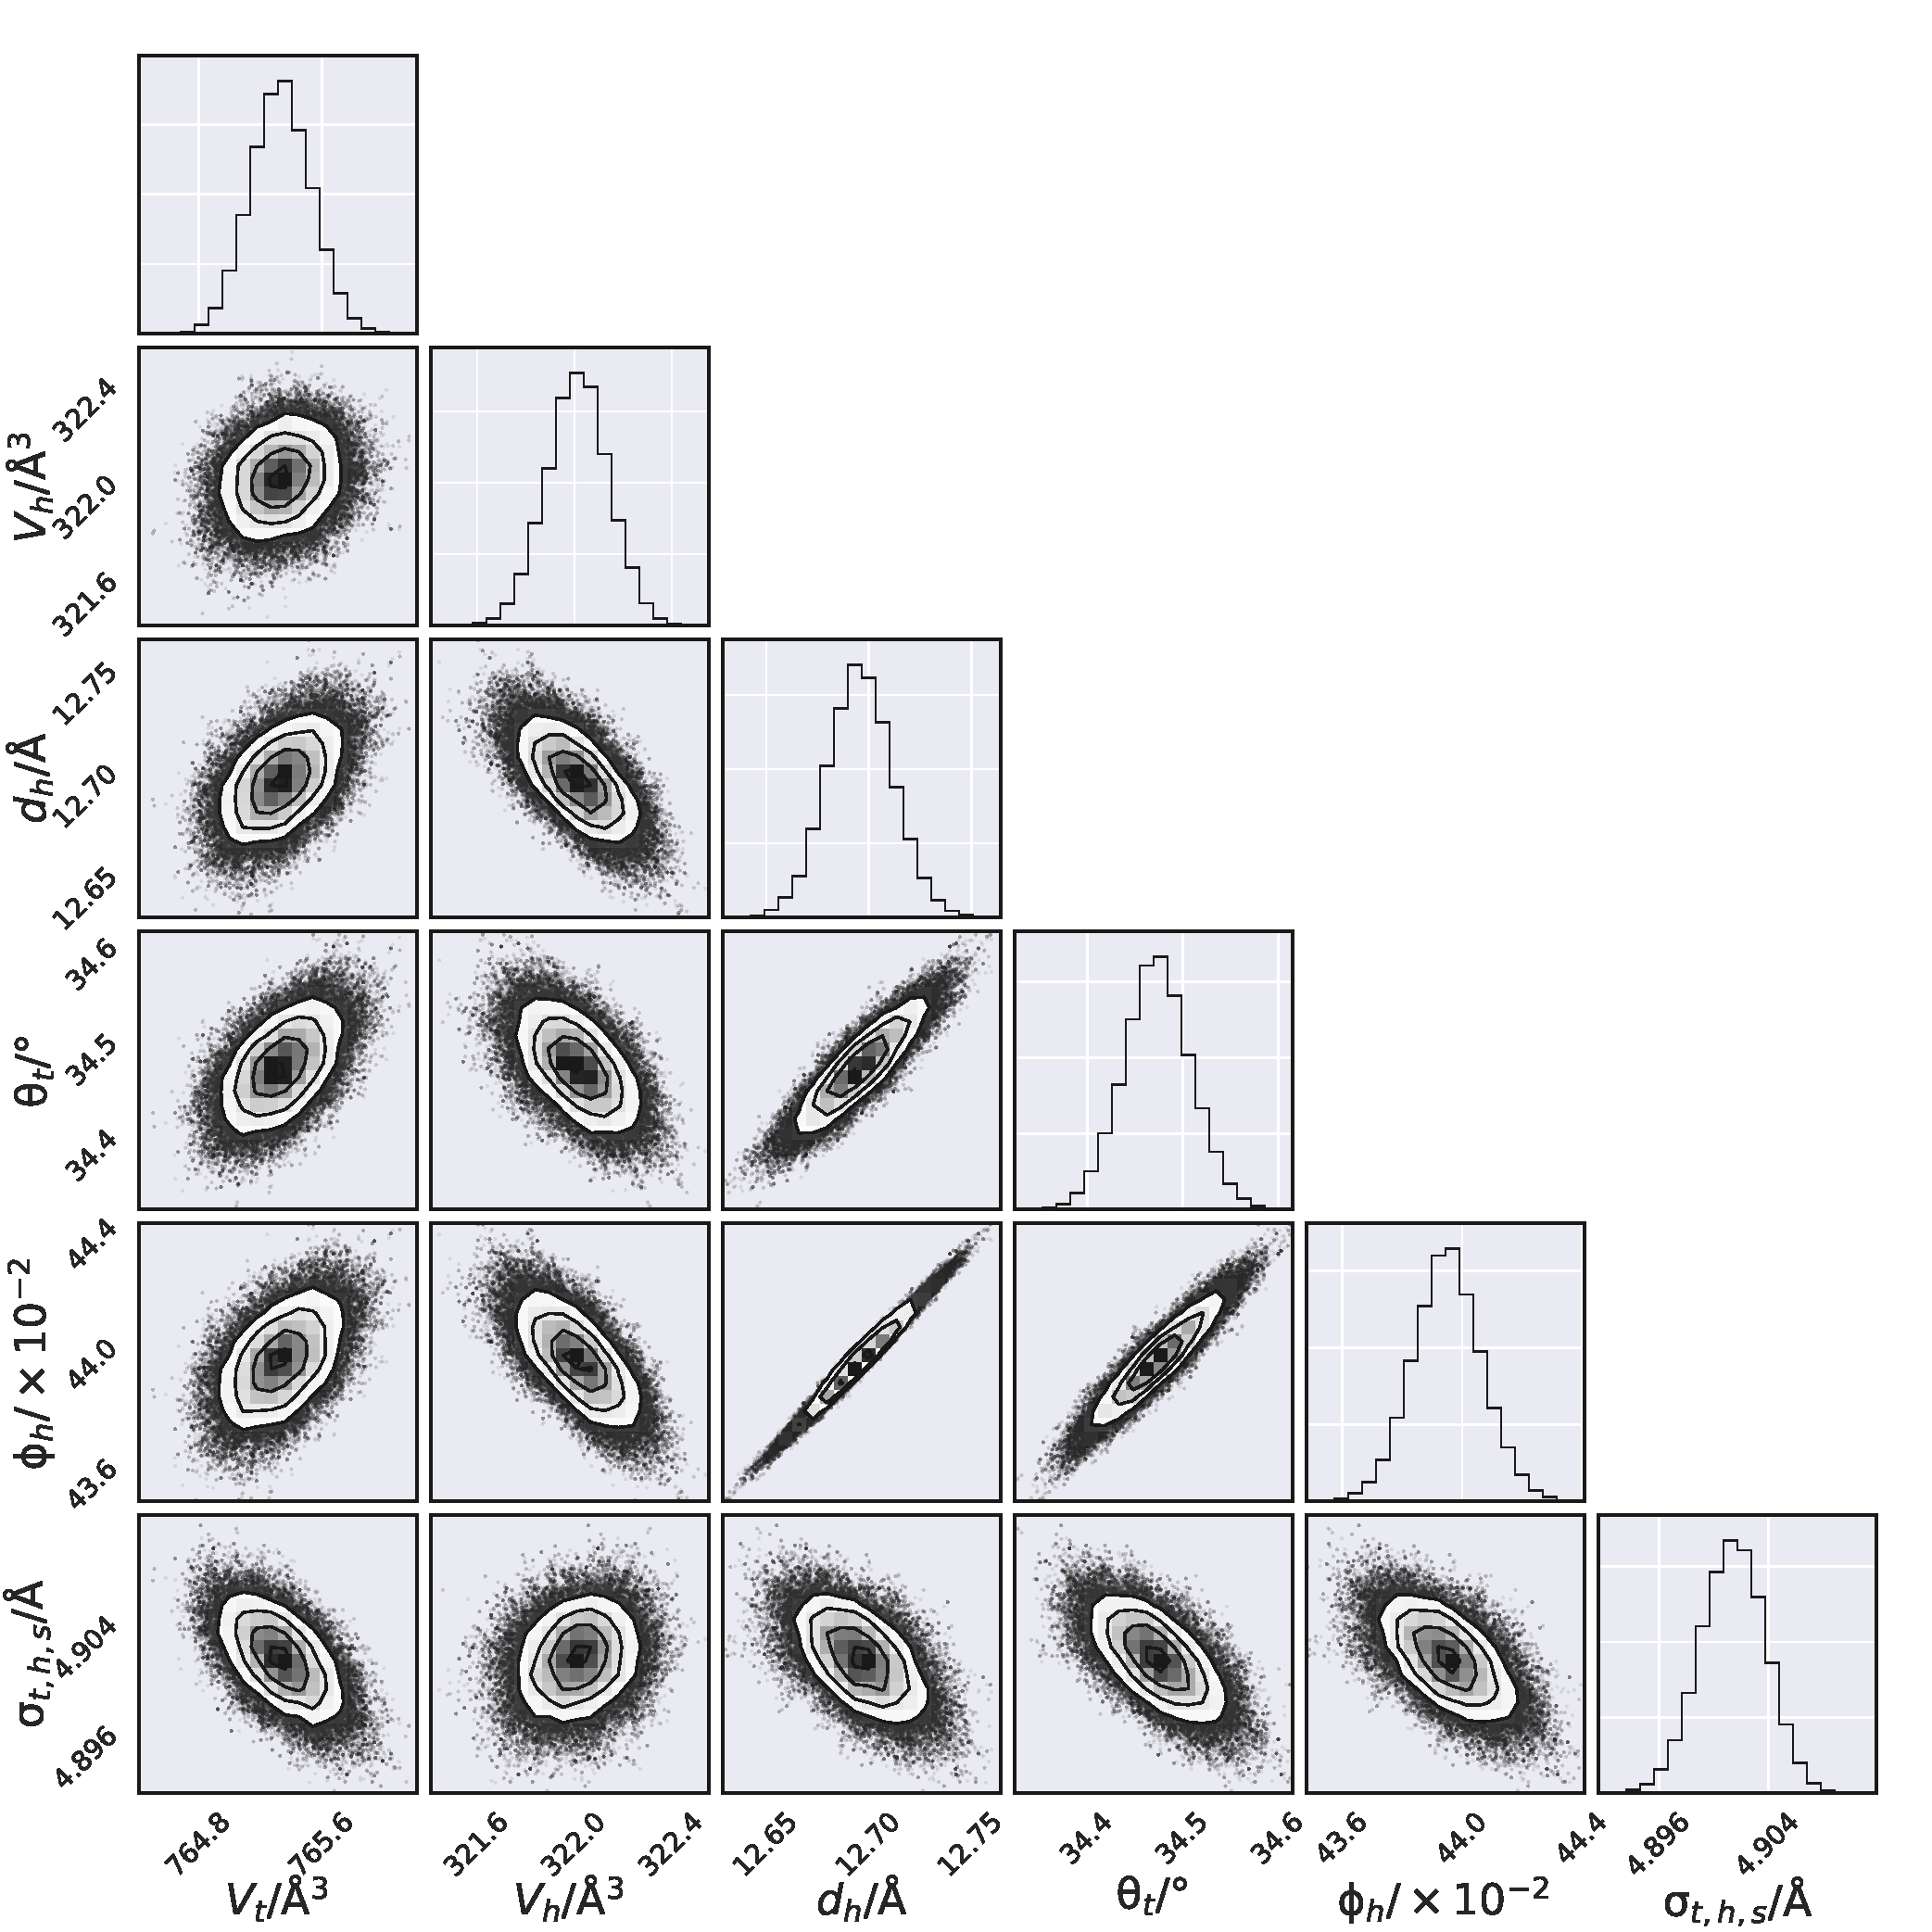
\includegraphics[width=0.50\textwidth]{figures/dppc5_all_corner}
	\caption{The multi-parameter PDFs for the chemically-relevant model of DPPC reflectometry data at the highest concentration. Figure files are available under MIT License.\cite{mccluskey_2018}}
	\label{fig:dppc5}
\end{figure}
\begin{figure}
	\centering
	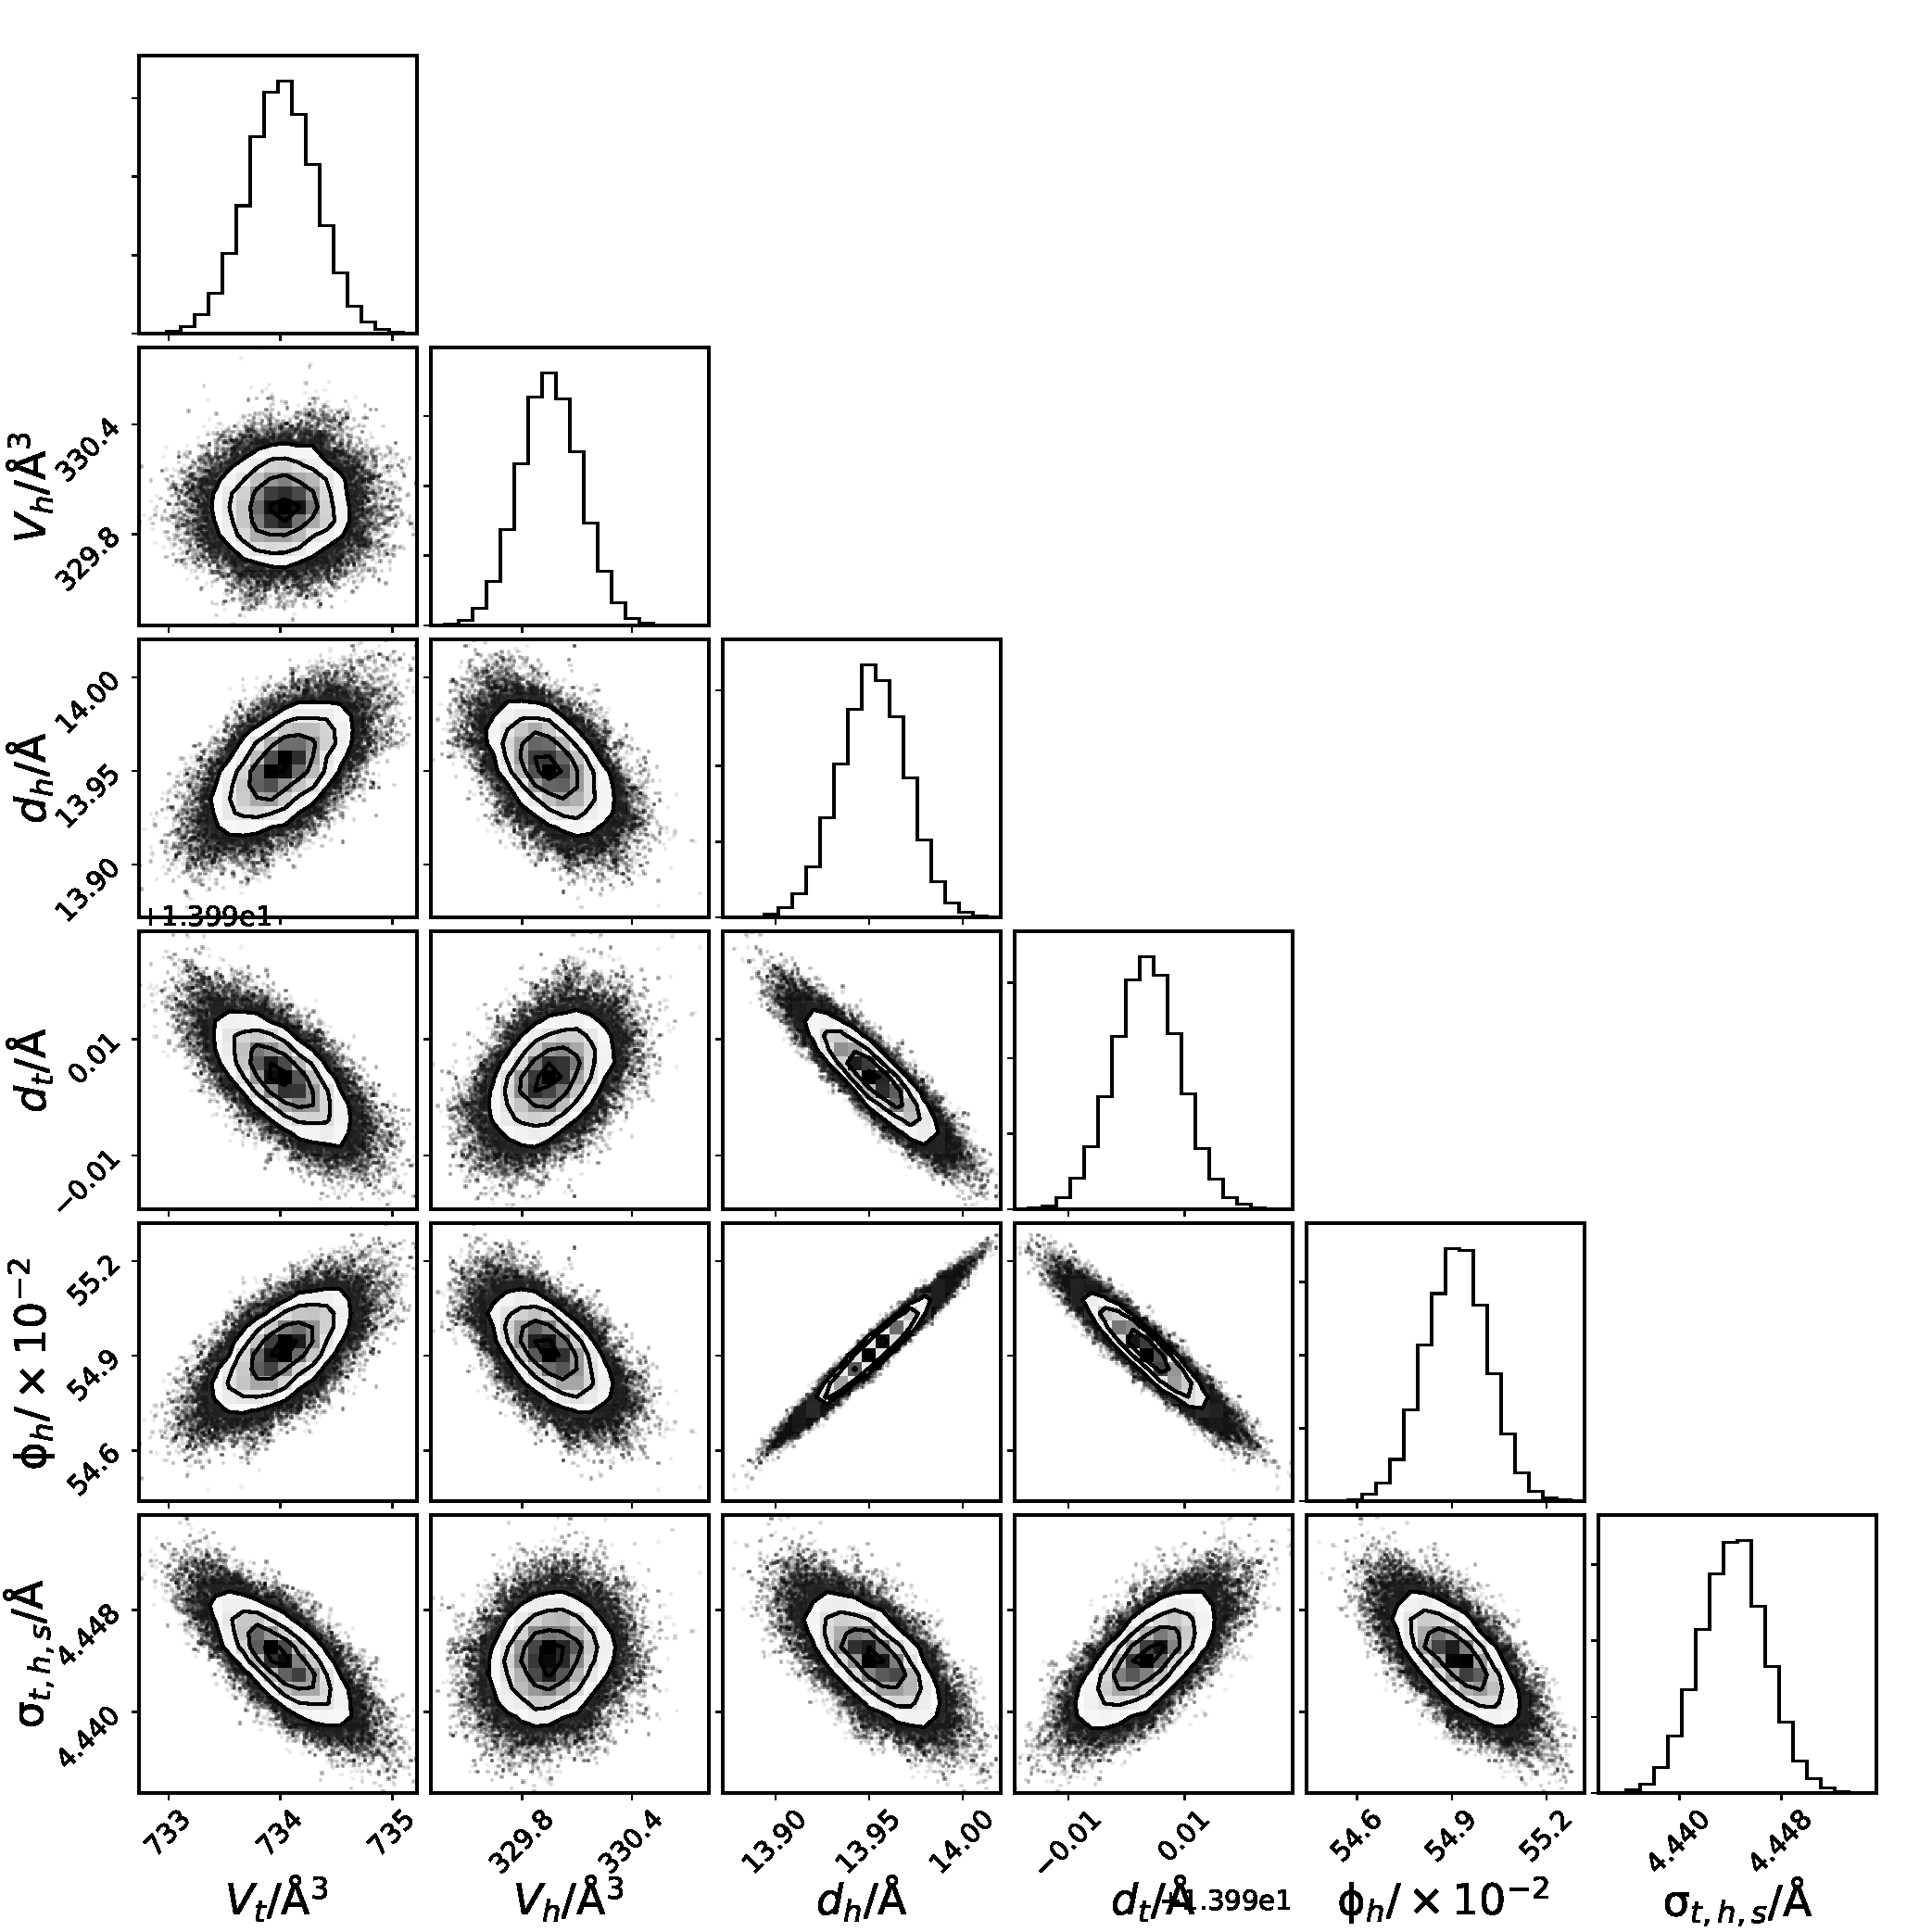
\includegraphics[width=0.50\textwidth]{figures/dmpg4_all_corner}
	\caption{The multi-parameter PDFs for the chemically-relevant model of DMPG reflectometry data at the second-highest concentration. Figure files are available under MIT License.\cite{mccluskey_2018}}
	\label{fig:dmpg4}
\end{figure}
\begin{figure}
	\centering
	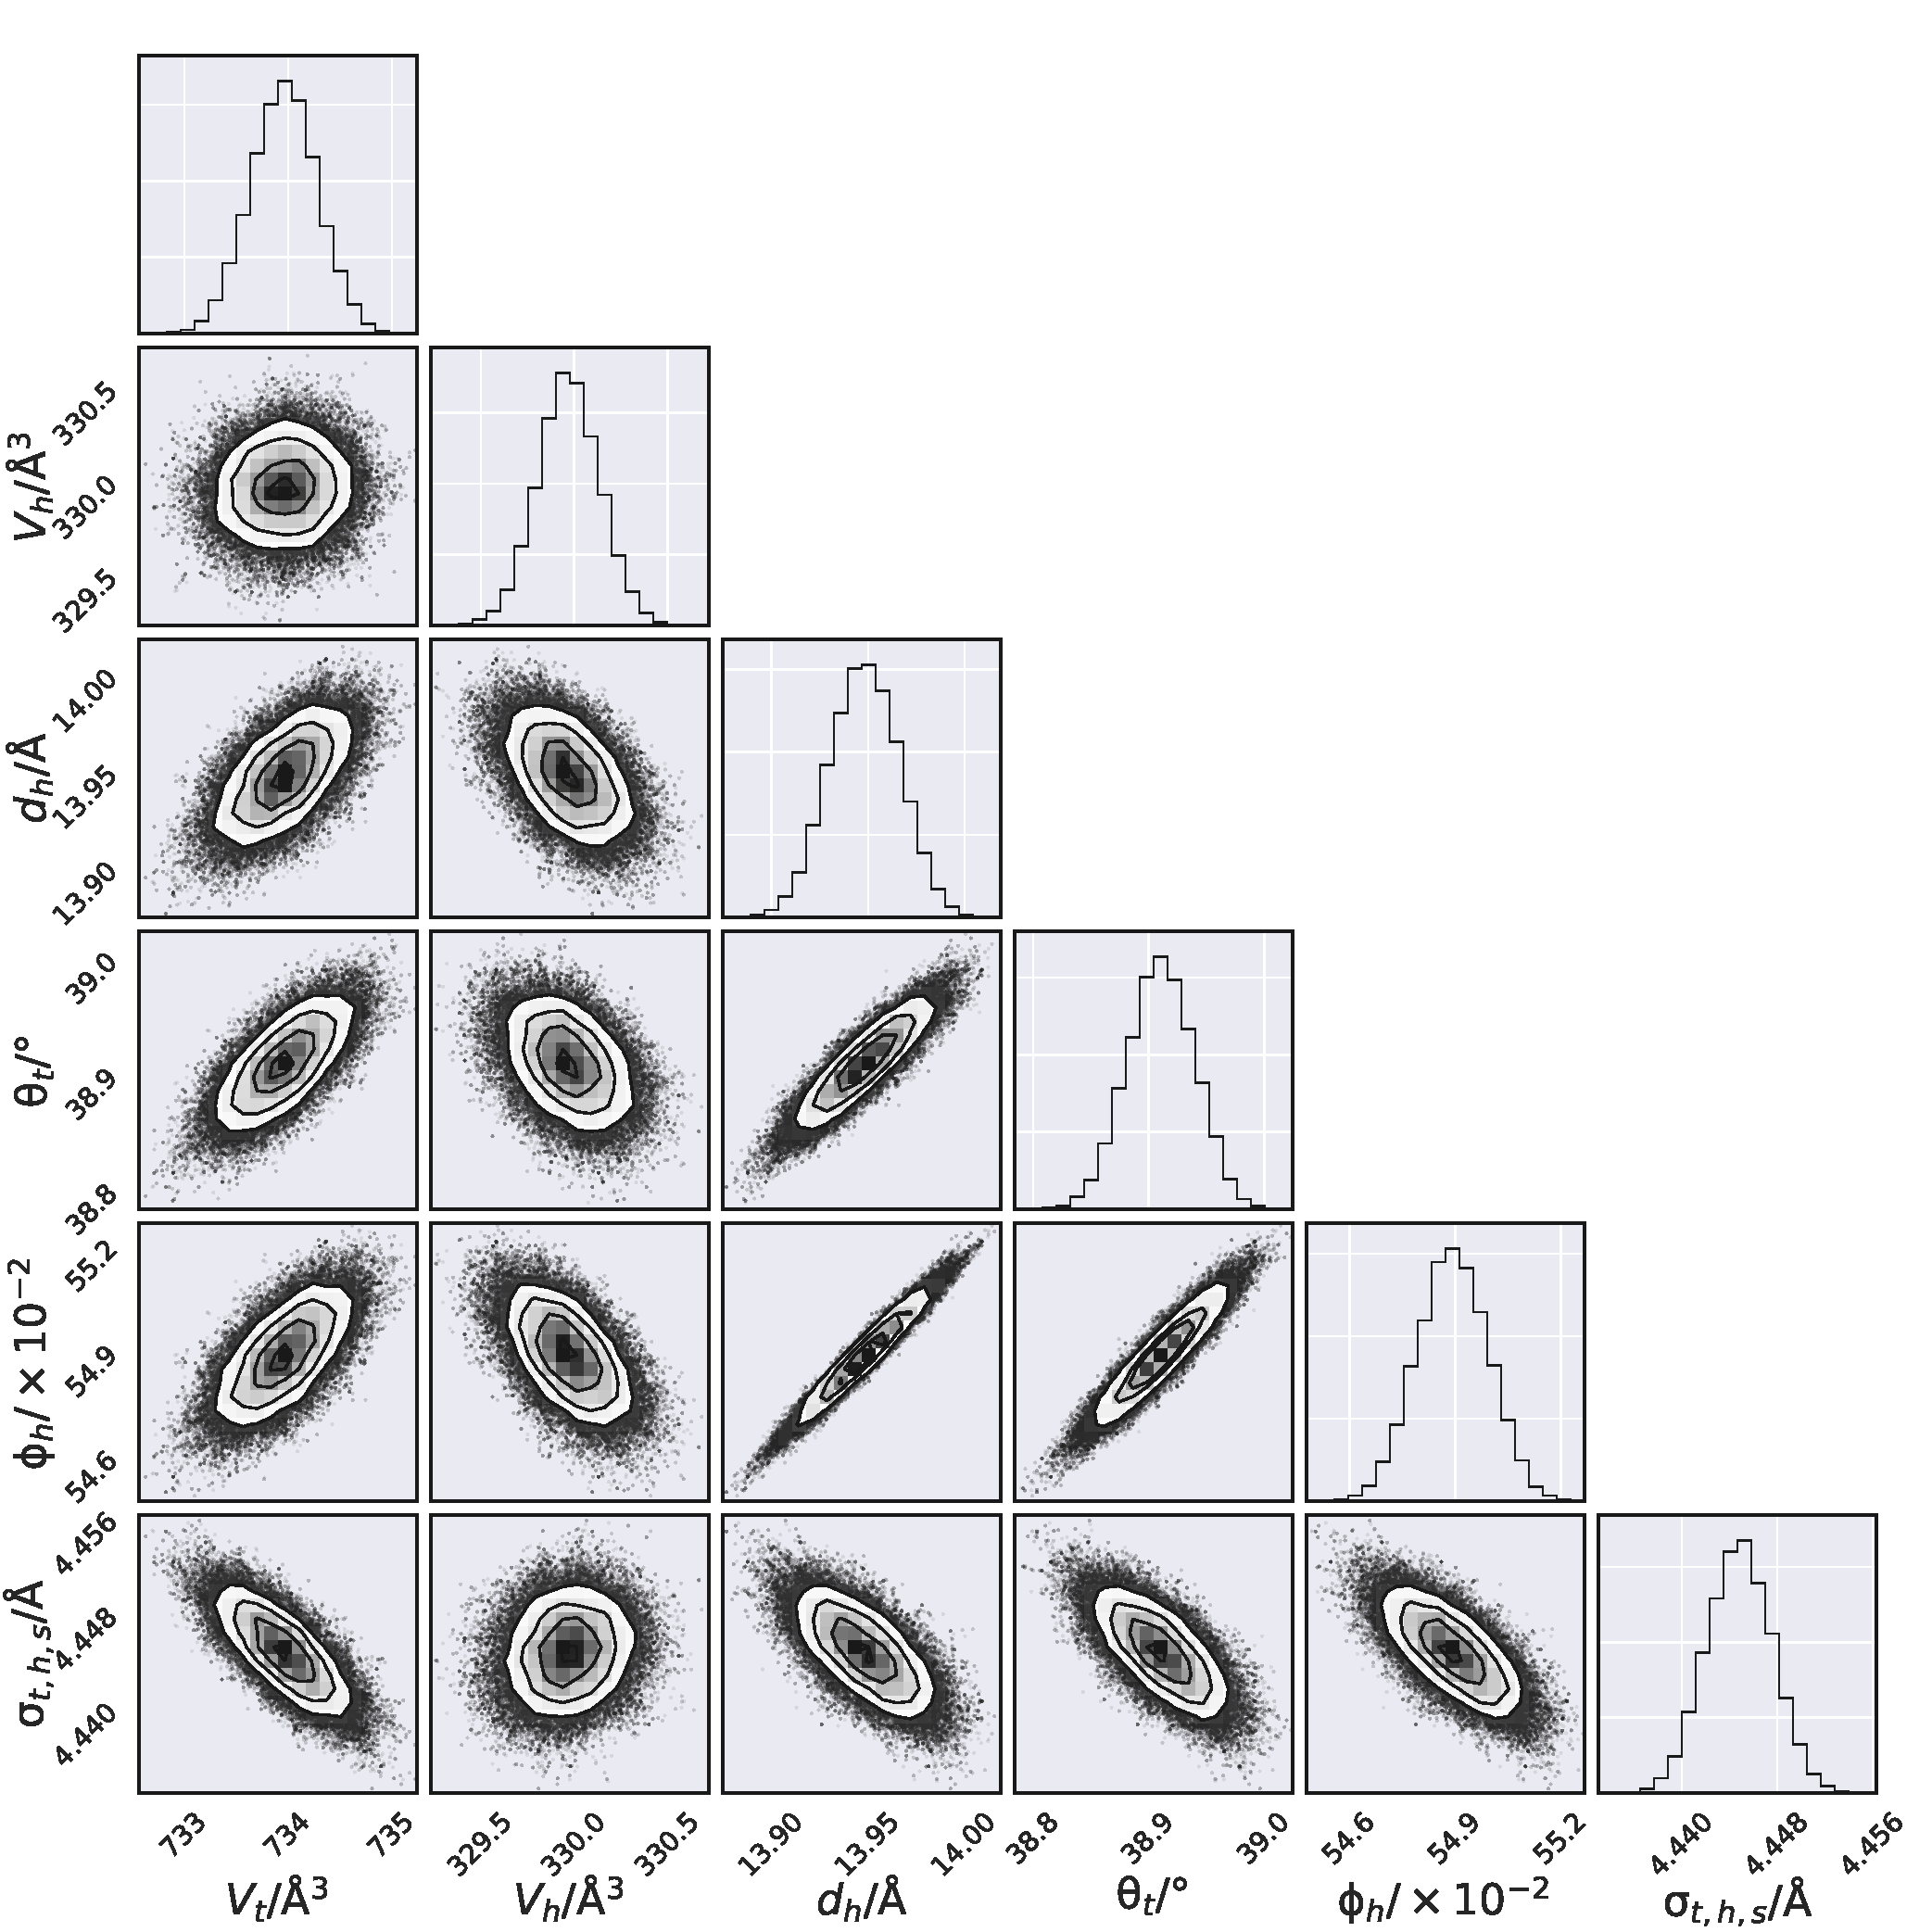
\includegraphics[width=0.50\textwidth]{figures/dmpg5_all_corner}
	\caption{The multi-parameter PDFs for the chemically-relevant model of DMPG reflectometry data at the highest concentration. Figure files are available under MIT License.\cite{mccluskey_2018}}
	\label{fig:dmpg5}
\end{figure}

	
%%%REFERENCES%%%
\bibliography{rsc} %You need to replace "rsc" on this line with the name of your .bib file
\bibliographystyle{rsc} %the RSC's .bst file
\end{document}